%This file is the main file where the final document is generated

\documentclass{these-ubl} 
\usepackage{bibunits}
\geometry{vmargin=4.0cm}

%Pour diff\'{e}rentes universit\'{e}s il faurdra modifier ce d\'{e}but de document
%For different universities modify the beginning of this document to adapt the logos (logo)
\geometry{vmargin=4.0cm}
\logoecoledoc{./Couverture-these/MathSTIC/logo-mathSTIC} %logo ecole doctorale
\logoetablissement{./Couverture-these/MathSTIC/logo-etablissements/logoUR1}%logo etablissement (ici Rennes 1) 
\vspace{2.5cm}
%Indiquer l'\'{e}tablissement de d\'{e}livrance du diplome
%Provide the name of the institution that delivers the diploma, 
\unite{L'UNIVERSIT\'{E} DE RENNES 1}
%Si la th\`{e}se est en co-tutelle ou en d\'{e}livrance conjointe, mettre le logo des 2 \'{e}tablissements 
%in the case of "co-tutelle" provide both names (logos)
\ubl{Comue Université Bretagne Loire}
%Indiquer le num\'{e}ro d’accr\'{e}ditation de l’\'{e}cole doctorale de r\'{e}f\'{e}rence pour la th\`{e}se 
%indicate the certification number of l'ecole doctorale
\ecoledoc{\'{E}cole Doctorale N° 601}
%Indiquer le nom de l’\'{e}cole doctorale de r\'{e}f\'{e}rence pour la th\`{e}se 
%Indicate the name of l'ecole doctorale
\nomecole{Math\'{e}matiques et Sciences et Technologies \\ de l'Information et de la Communication}
%Inscrivez ici votre sp\'{e}cialit\'{e} (voir liste des sp\'{e}cialit\'{e}s sur le site de votre \'{e}cole doctorale)
%Indicate the domain (see list of domains in your ecole doctorale)
\spec{Sp\'{e}cialit\'{e} : \textit{(voir liste des sp\'{e}cialit\'{e}s)}}
\usepackage{eso-pic}


\begin{document}

% PDF document Tags
\hypersetup{
    pdftitle={title},    % title
    pdfauthor={author},     % author
    pdfsubject={Subject},   % subject of the document
    pdfcreator={creator},   % creator of the document
    pdfproducer={producer}, % producer of the document
    pdfkeywords={Green Networking} {Mobile Cloud} {Network Coding} {Energy} % 
}

% La page de garde est en français
% The front cover is in French
\selectlanguage{french}

%background image of the front cover
\AddToShipoutPicture*{%
    \put(0,0){%
    \parbox[b][42.5cm]{\paperwidth}{%
        \vfill
        
\includegraphics[width=\paperwidth,keepaspectratio]{./Couverture-these/MathSTIC/image-fond-MATHSTIC-gardeO.png}% image de fond UR1
        \vfill
}}}
%Attention : le pr\'{e}nom doit être en minuscules (Jean) et le NOM en majuscules (BRITTEF) 
%Attention : the first name in small letters and the name in Capital letters 
\author{« Pr\'{e}nom NOM »}
% Donner le titre complet de la th\`{e}se, \'{e}ventuellement le sous titre, si n\'{e}cessaire sur plusieurs lignes 
%Give the complete title of the thesis, if necessary on several lines
\title{« Titre de la th\`{e}se »}
\lesoustitre{« Sous-titre de la th\`{e}se »}
%Indiquer la date et le lieu de soutenance de la th\`{e}se 
%indicates the date and the place of the defense 
\date{« date »}
\lieu{« Lieu »}
%Indiquer le nom du (ou des) laboratoire (s) dans le(s)quel(s) le travail de th\`{e}se a \'{e}t\'{e} effectu\'{e}, indiquer aussi si souhait\'{e} le nom de la (les) facult\'{e}(s) (UFR, \'{e}cole(s), Institut(s), Centre(s)...), son (leurs) adresse(s)... 
%Indicates the name (or names) of research laboratories where the work has been done as well as (if desired) the names of faculties (UFR, Schools, institution...
\uniterecherche{Unit\'{e} de recherche : }
%Indiquer le Numero de th\`{e}se, si cela est opportun, ou faire disparaitre cet item de la couverture 
%Indicate the number of the thesis if there is one.
\numthese{Th\`{e}se N° :  }
%Indiquer le Pr\'{e}nom en minuscules et le Nom en majuscules, le titre de la personne et l’\'{e}tablissement dans lequel il effectue sa recherche  
%Indicates the first name on small letters and the Names on capital letters, the person's title and the institution where he/she belongs to.
%Exemples :  Examples :
%%%- Professeur, Universit\'{e} d’Angers 
%%%- Chercheur, CNRS, \'{e}cole Centrale de Nantes 
%%%-  Professeur d’universit\'{e} – Praticien Hospitalier, Universit\'{e} Paris V  
%%%-  Maitre de conf\'{e}rences, Oniris 
%%%- Charg\'{e} de recherche, INSERM, HDR, Universit\'{e} de Tours  
 %S’il n’y a pas de co-direction, faire disparaitre cet item de la couverture  
 %In there is no co-director, remove the item from the cover


\jury{
{\normalsize \textbf{Rapporteurs avant soutenance :}}\\
\begin{tabular}{@{}ll}
Pr\'{e}nom Nom & Fonction et \'{e}tablissement d'exercice \\
Pr\'{e}nom Nom & Fonction et \'{e}tablissement d'exercice \\
Pr\'{e}nom Nom & Fonction et \'{e}tablissement d'exercice \\
\end{tabular}

\vspace{\baselineskip}
{\normalsize \textbf{Composition du Jury :}}\\
{\textcolor{red}{\textit{Attention, en cas d’absence d’un des membres du Jury le jour de la soutenance, la composition du Jury}}}\\
{\textcolor{red}{\textit{ne comprend que les membres pr\'{e}sents}}}\\
\begin{tabular}{@{}lll}

Pr\'{e}sident :        & Pr\'{e}nom Nom & Fonction et \'{e}tablissement d'exercice \textit{(à préciser après la soutenance)} \\
Examinateurs :         & Pr\'{e}nom Nom & Fonction et \'{e}tablissement d'exercice \\
                       & Pr\'{e}nom Nom & Fonction et \'{e}tablissement d'exercice \\
                       & Pr\'{e}nom Nom & Fonction et \'{e}tablissement d'exercice \\
                       & Pr\'{e}nom Nom & Fonction et \'{e}tablissement d'exercice \\
Dir. de th\`{e}se :    & Pr\'{e}nom Nom & Fonction et \'{e}tablissement d'exercice \\
Co-dir. de th\`{e}se : & Pr\'{e}nom Nom & Fonction et \'{e}tablissement d'exercice \textit{(si pertinent)} \\
\end{tabular}

\vspace{\baselineskip}
{\normalsize \textbf{Invit\'{e}(s) :}}\\
\begin{tabular}{@{}ll}
Pr\'{e}nom Nom & Fonction et \'{e}tablissement d'exercice \\
\end{tabular}
}


\maketitle
 % page de garde UR1

% Select the content language following this line
\selectlanguage{english}

%input acknowledgement chapter 
\clearemptydoublepage
\chapter*{Acknowledgement}

Je tiens à remercier  \\
I would like to thank. my parents..\\
J'adresse également toute ma reconnaissance à .... \\
....


%Inut resume en Francais
\clearemptydoublepage
\begin{bibunit}[IEEEtran.bst]

\chapter*{Résumé en français}

\section*{Motivations}

\section*{Objectifs}

\section*{Contributions}

\section*{Contenu du manuscrit}

In this manuscript I'd like to cite \cite{remo1,remo2}.

\putbib[./Resume-Francais/Res-Biblio.bib]
\end{bibunit}

%This command will generate the front cover
\clearemptydoublepage
\frontmatter 
\renewcommand{\contentsname}{Table of Contents}
\setcounter{tocdepth}{5}
\tableofcontents %sommaire %table of content

\clearemptydoublepage
\chapter*{List of acronyms}
\addcontentsline{toc}{chapter}{List of acronyms}
\chaptermark{List of acronyms}


\begin{tabular}{ll}
AA & Active Alert \\
AAM & Active Appearance Models \\
ANN & Artificial Neural Networks \\
APSS & Association of the Psychophysiological Study of Sleep \\ 
AR & Auto Regressive \\
AS & Active Sleep \\
AU & Action Unit \\
AUC & Area Under Curve \\
B\&W & Black and White \\
CCHS & Congenital Central Hypoventilation Syndrome \\
CNN & Convolution Neural Networks \\
CNS & Central Nervous System \\
CP & Cerebral Palsy \\
CU & Cry Unit \\
CWT & Continuous Wavelet Transform \\
D & Drowsiness \\
DAN & Douleur Aig{\"u}e du Nouveau-n{\'e} \\
DCT & Discrete Cosinus Transform \\

\end{tabular}

\begin{tabular}{ll}
KLT & Kanade-Lucas-Tomasi \\
KNN & K-Nearest Neighbors \\
LDA & Linear Discriminant Analysis \\
LOOCV & Leave-one-out cross-validation \\
LPCCs & Linear Prediction Cepstral Coefficients \\
LR & Logistic Regression \\
LTAS & Long Time Average Spectrum \\
MFCCs & Mel Frequency Cepstral Coefficients \\
MLE & Maximum Likelihood Estimation \\
MLP & Multi-Layer Perceptron \\
NBAS & Neonatal Behavioral Assessment Scale \\
NFCS & Neonatal Facial Coding System \\
NICU & Neonatal Intensive Care Units\\
NIDCAP & Newborn Individualized Developmental Care and Assessment Program  \\
NIR & Near-InfraRed \\
NLEO & Non Linear Energy Operator \\
NUC & Next Unit of Computing \\
OSA & Obstructive Sleep Apnea \\
PCA & Principal Component Analysis \\
PMA & PostMenstrual Age \\


\end{tabular}




\listoffigures
\addcontentsline{toc}{chapter}{List of figures}

\listoftables
\addcontentsline{toc}{chapter}{List of tables} 

\clearemptydoublepage
\begin{bibunit}[IEEEtran.bst]

\chapter*{Introduction}
\addcontentsline{toc}{chapter}{Introduction}
\chaptermark{Introduction}

Lorem ipsum dolor sit amet, «~consectetuer~» adipiscing elit. Maecenas fermentum, elit non lobortis cursus, orci velit suscipit est, id mollis turpis mi eget orci.

Lorem ipsum dolor sit amet, consectetuer adipiscing elit. Maecenas fermentum, elit non lobortis cursus, orci velit suscipit est, id mollis turpis mi eget orci.

\section*{Première section de l'introduction}
\addcontentsline{toc}{section}{Première section de l'intro}

Lorem ipsum dolor sit amet, «~consectetuer~» adipiscing elit. Maecenas fermentum, elit non lobortis cursus, orci velit suscipit est, id mollis turpis mi eget orci.

\textbf{Une boite magique : }

\boitemagique{Titre de la boite}{
Praesent placerat, ante at venenatis pretium, diam turpis faucibus arcu, nec vehicula quam lorem ut leo. Sed facilisis, augue in pharetra dapibus, ligula justo accumsan massa, eu suscipit felis ipsum eget enim.
}

Laoreet iaculis, nonummy eget, massa. Phasellus ullamcorper commodo velit. Class aptent taciti sociosqu ad litora torquent per «~conubia nostra~», per inceptos hymenaeos. Phasellus est. Maecenas felis augue, gravida quis, porta adipiscing, iaculis vitae, felis.

\textbf{Une boite simple : }
\boitesimple{Mauris lorem quam, tristique sollicitudin egestas sed, sodales vel leo. In hac habitasse platea dictumst. Lorem ipsum dolor sit amet, consectetur adipiscing elit. Sed sed lorem lacus, at venenatis elit. Pellentesque nisl arcu, blandit ac eleifend non, sodales a quam.}

Laoreet iaculis, nonummy eget, massa. Phasellus ullamcorper commodo velit.

% In this manuscript I'd like to cite \cite{remo1,remo2}.

% \addcontentsline{toc}{section}{Bibliography}
% \putbib[./Introduction/Intro-Biblio.bib]
\end{bibunit}

%\shorttableofcontents{Sommaire}{0}

\clearemptydoublepage
\mainmatter % Ne pas oublier, avec \frontmatter et \backmatter
	           %this command inputs \frontmatter and \backmatter as a cover in the front and the back

%Input your chapter 1
\begin{bibunit}[IEEEtran.bst]

\clearemptydoublepage
\chapter{Titre du premier chapitre}

Lorem ipsum dolor sit amet, consectetuer adipiscing elit. Maecenas fermentum, elit non lobortis cursus, orci velit suscipit est, id mollis turpis mi eget orci.

\section{Première section du chapitre}

Lorem ipsum dolor sit amet, consectetuer adipiscing elit. Maecenas fermentum, elit non lobortis cursus, orci velit suscipit est, id mollis turpis mi eget orci.

\subsection{Première sous-section}

Lorem ipsum dolor sit amet, consectetuer adipiscing elit. Maecenas fermentum, elit non lobortis cursus, orci velit suscipit est, id mollis turpis mi eget orci.

Voir figure \ref{fig:mafigure2}.


\begin{figure}[htbp]
   \begin{center}
      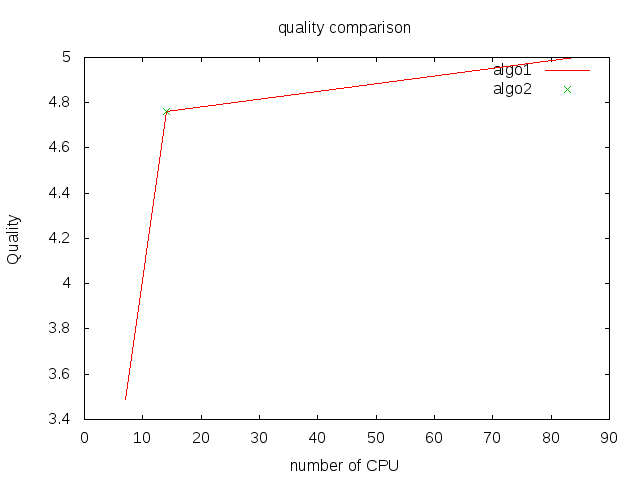
\includegraphics[width=0.8\linewidth]{Chapitre1/Ch1-Figures/comparison.png}
   \end{center}
   \caption[titre court pour la liste des figures]
   {\footnotesize Titre plus long avec des explications.}
   \label{fig:mafigure2}
\end{figure}

\subsection{Deuxième sous-section}

Lorem ipsum dolor sit amet, consectetuer adipiscing elit. Maecenas fermentum, elit non lobortis cursus, orci velit suscipit est, id mollis turpis mi eget orci.

\section{Conclusion du premier chapitre}

Lorem ipsum dolor sit amet, consectetuer adipiscing elit. Maecenas fermentum, elit non lobortis cursus, orci velit suscipit est, id mollis turpis mi eget orci.

In this manuscript I'd like to cite \cite{remo3,remo4}.

\addcontentsline{toc}{section}{Bibliography}
\putbib[./Chapitre1/Ch1-Biblio.bib]
\end{bibunit}


%Input your chapter 2
\clearemptydoublepage
\begin{bibunit}[IEEEtran.bst]

\chapter[SHORT-Nom-du-chapitre-2]{Nom du chapitre 2}

Lorem ipsum dolor sit amet, consectetuer adipiscing elit. Maecenas fermentum, elit non lobortis cursus, orci velit suscipit est, id mollis turpis mi eget orci. 

\section{Première section du chapitre}

\subsection{Première sous-section}

Morbi lorem. Etiam scelerisque rhoncus orci. Nunc elementum ante ac leo. Vestibulum venenatis dictum nunc. Donec turpis est, dictum nec, fringilla nec, cursus id, quam. In nibh orci, porttitor ut, rutrum id, faucibus vitae, leo. Donec ut wisi.

\subsection{Deuxième sous-section}

Lorem ipsum dolor sit amet, consectetuer adipiscing elit. Maecenas fermentum, elit non lobortis cursus, orci velit suscipit est, id mollis turpis mi eget orci. Table \ref{table1}.

\begin{table}[hbt]
\begin{center}
\begin{tabular}{|l|l|l|}
\hline
A & B & C \\ \hline
D & E & F \\ \hline
G & H & I \\ \hline
\end{tabular}
\caption{Test Table}
\label{table1}
\end{center}
\end{table}

\section{Conclusion du second chapitre}

Lorem ipsum dolor sit amet, consectetuer adipiscing elit. Maecenas fermentum, elit non lobortis cursus, orci velit suscipit est, id mollis turpis mi eget orci.

In this manuscript I'd like to cite \cite{remo1,remo5}.

\addcontentsline{toc}{section}{Bibliography}
\putbib[./Chapitre2/Ch2-Biblio.bib]
\end{bibunit}

\clearemptydoublepage
\backmatter
\begin{bibunit}[IEEEtran.bst]

\chapter*{Conclusions and perspectives}
\label{chap:conclusions}
\addcontentsline{toc}{chapter}{Conclusion and perspectives}
\chaptermark{Conclusion}

Lorem ipsum dolor sit amet, consectetuer adipiscing elit. Maecenas fermentum, elit non lobortis cursus, orci velit suscipit est, id mollis turpis mi eget orci.

\section*{Première section de la conclusion}
\addcontentsline{toc}{section}{Première section de la conclusion}

Lorem ipsum dolor sit amet, consectetuer adipiscing elit. Maecenas fermentum, elit non lobortis cursus, orci velit suscipit est, id mollis turpis mi eget orci.

Lorem ipsum dolor sit amet, consectetuer adipiscing elit. Maecenas fermentum, elit non lobortis cursus, orci velit suscipit est, id mollis turpis mi eget orci.

% \addcontentsline{toc}{section}{Bibliography}
% \putbib[./Conclusion/End-Biblio.bib]
\end{bibunit}

% \clearemptydoublepage
\addcontentsline{toc}{chapter}{List of publications}

% \chapter*{List of publications}
% \section*{International Journals}
% \section*{International Conferences}

\begin{bibunit}[IEEEtran.bst]
\renewcommand\bibname{List of publications}
\nocite{*}
\putbib[./PublicationList/PubList-Biblio.bib]
\end{bibunit}





\clearemptydoublepage
\begin{bibunit}[IEEEtran.bst]

\chapter*{Appendix}
\addcontentsline{toc}{chapter}{Appendix}

\section*{User Guide}
\addcontentsline{toc}{section}{User Guide}

% \addcontentsline{toc}{section}{Bibliography}
% \putbib[./Appendix/App-Biblio.bib]
\end{bibunit}


\clearemptydoublepage
% Pour avoir la quatrième de couverture sur une page paire
% To have the back cover on an even page
\cleartoevenpage[\thispagestyle{empty}]
\markboth{}{}
% Plus petite marge du bas pour la quatrième de couverture
% Shorter bottom margin for the back cover
\newgeometry{inner=30mm,outer=20mm,top=40mm,bottom=20mm}

%insertion de l'image de fond du dos (resume)
%background image for resume (back)
\backcoverheader

% Switch font style to back cover style
\selectfontbackcover{ % Font style change is limited to this page using braces, just in case

\titleFR{titre (en fran\c cais)..............}

\keywordsFR{de 3 \`{a} 6 mots clefs}

\abstractFR{Eius populus ab incunabulis primis ad usque pueritiae tempus extremum, quod annis circumcluditur fere trecentis, circummurana pertulit bella, deinde aetatem ingressus adultam post multiplices bellorum aerumnas Alpes transcendit et fretum, in iuvenem erectus et virum ex omni plaga quam orbis ambit inmensus, reportavit laureas et triumphos, iamque vergens in senium et nomine solo aliquotiens vincens ad tranquilliora vitae discessit.
Hoc inmaturo interitu ipse quoque sui pertaesus excessit e vita aetatis nono anno atque vicensimo cum quadriennio imperasset. natus apud Tuscos in Massa Veternensi, patre Constantio Constantini fratre imperatoris, matreque Galla.
Thalassius vero ea tempestate praefectus praetorio praesens ipse quoque adrogantis ingenii, considerans incitationem eius ad multorum augeri discrimina, non maturitate vel consiliis mitigabat, ut aliquotiens celsae potestates iras principum molliverunt, sed adversando iurgandoque cum parum congrueret, eum ad rabiem potius evibrabat, Augustum actus eius exaggerando creberrime
docens, idque, incertum qua mente, ne lateret adfectans. quibus mox Caesar acrius efferatus, velut contumaciae quoddam vexillum altius erigens, sine respectu salutis alienae vel suae ad vertenda opposita instar rapidi fluminis irrevocabili impetu ferebatur.
Hae duae provinciae bello quondam piratico catervis mixtae praedonum.}



\titleEN{titre (en anglais)..............}

\keywordsEN{de 3 \`{a} 6 mots clefs}

\abstractEN{Eius populus ab incunabulis primis ad usque pueritiae tempus extremum, quod annis circumcluditur fere trecentis, circummurana pertulit bella, deinde aetatem ingressus adultam post multiplices bellorum aerumnas Alpes transcendit et fretum, in iuvenem erectus et virum ex omni plaga quam orbis ambit inmensus, reportavit laureas et triumphos, iamque vergens in senium et nomine solo aliquotiens vincens ad tranquilliora vitae discessit.
Hoc inmaturo interitu ipse quoque sui pertaesus excessit e vita aetatis nono anno atque vicensimo cum quadriennio imperasset. natus apud Tuscos in Massa Veternensi, patre Constantio Constantini fratre imperatoris, matreque Galla.
Thalassius vero ea tempestate praefectus praetorio praesens ipse quoque adrogantis ingenii, considerans incitationem eius ad multorum augeri discrimina, non maturitate vel consiliis mitigabat, ut aliquotiens celsae potestates iras principum molliverunt, sed adversando iurgandoque cum parum congrueret, eum ad rabiem potius evibrabat, Augustum actus eius exaggerando creberrime
docens, idque, incertum qua mente, ne lateret adfectans. quibus mox Caesar acrius efferatus, velut contumaciae quoddam vexillum altius erigens, sine respectu salutis alienae vel suae ad vertenda opposita instar rapidi fluminis irrevocabili impetu ferebatur.
Hae duae provinciae bello quondam piratico catervis mixtae praedonum.}

}

% Rétablit les marges d'origines
% Restore original margin settings
\restoregeometry

\end{document}
